\section{\red{Problem Statement}}
\label{sec:problem}

\subsection{\red{System Setting}}

\red{We formalize post-training federation. We distinguish package owners from deployment sites, although one organization may have both roles. Before collaboration, each owner freezes a detector and registers it. A trusted registry distributes the same versioned package pool to every site. The registry checks that each package matches the registered version, but it does not certify its behavior. During collaboration, the sites run the packages locally, while a separate coordinator trains a shared composer from secure aggregates.}

\red{More formally, we consider $J\ge2$ deployment sites that reuse $m$ intrusion detectors. Every package follows the same input and class-score interface over $C$ classes. For detector $i$, we write its frozen package and valid score output as}
\begin{equation}
\red{\mathcal M_i=(T_i,f_i), \qquad q_i(x)=f_i(T_i(x))\in\Delta^{C-1},}
\label{eq:frozen_package}
\end{equation}
\red{where $T_i$ and $f_i$ form the fixed inference pipeline, and $q_i$ is its normalized class-score output. We keep $T_i$ and $f_i$ fixed.}

\red{To identify the package deployed at each site, we use the map $\iota:\{1,\ldots,J\}\rightarrow\{1,\ldots,m\}$. At site $D_j$, the deployed package produces}
\begin{equation}
\red{b_j(x)=q_{\iota(j)}(x)}
\label{eq:incumbent}
\end{equation}
\red{and we call $b_j$ the raw incumbent output. A site may deploy a package from another organization, so we do not require $m=J$. The audit later compares its candidate with a fixed transformation of $b_j$. We call this comparator the audited incumbent and define it in Section~\ref{sec:approach}.}

\red{We call the labeled local observations obtained from the package pool \emph{current site data}. For fitting and audit, each site divides these data into a nonempty fit set $B_j^{fit}$ and a held-out audit set $B_j^{safe}$. We use $B_j^{fit}$ for shared training and local personalization, and we also use it to fix every audit choice. We reserve $B_j^{safe}$ for the final adoption audit. We do not assume that the current site distribution matches the unknown training distribution of any package.}

\red{During shared training, each site keeps its per-example current site data local and submits its composer gradient through secure aggregation. Local personalization and the adoption audit send no message to the coordinator.}

\subsection{\red{Problem Formulation}}

\red{Given the frozen package pool and current site data, each site needs both a candidate and an authorization decision. Candidate construction uses only the fit sets and seeks to reduce site-level fit loss by sharing correction structure when it is useful. Authorization is a separate constraint: site $j$ preselects a nonempty set of audit metrics $\mathcal E_j$ and a tolerance $\eta_{j,e}$ for every $e\in\mathcal E_j$, then deploys the frozen candidate only when a valid local audit places an upper bound on its excess risk over the audited incumbent within every tolerance. Thus, construction searches for utility without access to the audit set, while authorization determines whether that candidate may replace the incumbent.}

\subsection{\red{Threat Model}}
\label{sec:threat_model}

\red{We consider an honest-but-curious coordinator as the privacy adversary. It follows the prescribed protocol but may analyze its training view across rounds. In each completed round, this view includes the decoded aggregate gradient and the resulting shared composer. The coordinator receives no message from local personalization or the adoption audit.}

\red{We assume that the deployment sites follow the protocol and that none colludes with the coordinator. We also assume the standard authenticated communication required by secure aggregation. We trust the registry only to distribute the same registered pool to every site. Each site verifies this pool and runs its packages unchanged. We make no accuracy assumption about a package, but we model it as a fixed inference function. Executable code that violates this model is outside our scope.}

\red{For adoption, we assume that the held-out labels are correct for the audited task and fixed independently of the candidate. A systematic labeling error changes the risk controlled by our result.}

\red{Under these assumptions, per-example current site data remain local, and the coordinator does not receive any site's encoded composer gradient in plaintext. However, the shared composer may still leak information, and we provide no differential privacy. We do not protect against inference by another site or against active protocol deviations. Finally, because deployment sites execute the packages locally, we do not hide the packages from them.}


\section{\red{Design of \Fname}}
\label{sec:approach}

\begin{figure*}[htbp]
    \centering
    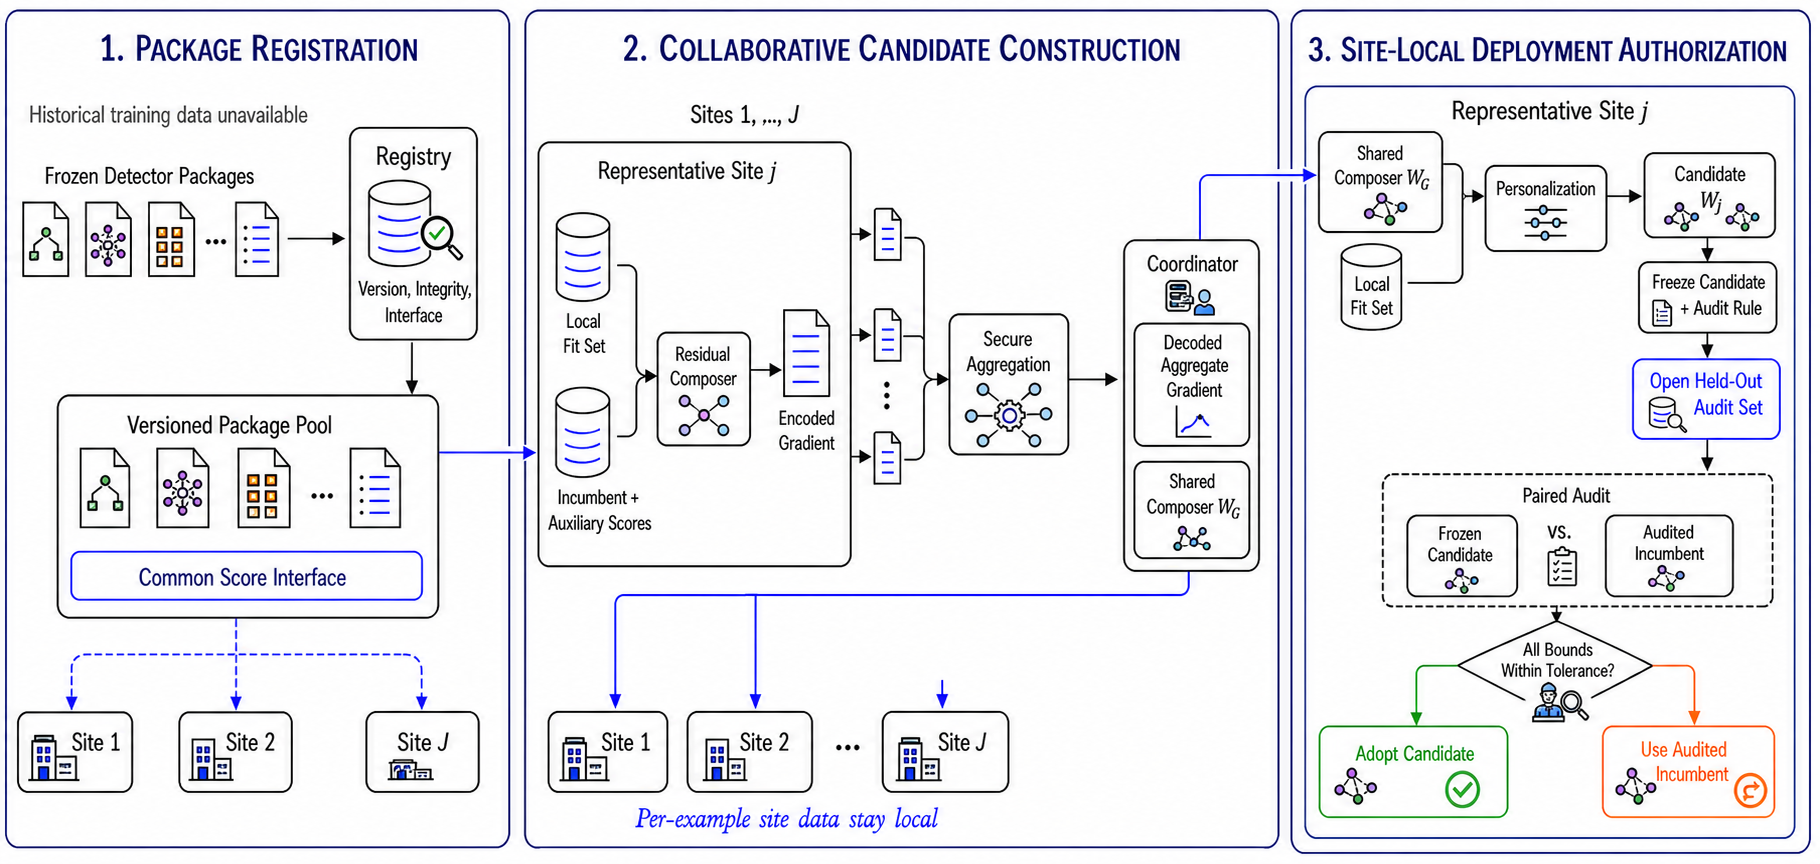
\includegraphics[width=\linewidth]{figures/post-training-federation-overview-v4.png}
    \caption{\red{Overview of \Fname through deployment authorization. Each site learns a personalized composer and audits it before deployment. The coordinator receives aggregated composer gradients, while each site keeps per-example scores and its personalized composer local. Section~\ref{sec:approach} describes the separate runtime response after authorization.}}
    \label{fig:workflow}
\end{figure*}

\subsection{\red{Overview}}

\red{Even without its historical training material, an auxiliary detector may help correct incumbent errors on current site data. We therefore compose only final scores and learn corrections relative to the incumbent. This design gives the sites a common correction space and retains an exact no-change state. When correction structure is shared, federated training can pool signals across sites and provide a common prior. However, package utility may differ by site, so the shared composer remains a starting point for local personalization. The resulting predictor remains a candidate until a held-out audit authorizes its deployment. Candidate construction and deployment authorization are therefore separate by design: collaboration can change the candidate, but only the local audit can change deployment.}

\red{As shown in Figure~\ref{fig:workflow}, the workflow begins with package registration. Before fitting, every site verifies the complete pool manifest. If any site finds a mismatch, the collaboration stops and the sites keep their existing deployments. Each site then builds incumbent-anchored inputs from $B_j^{fit}$ and trains the shared composer from securely aggregated, encoded gradients. After the coordinator returns $W_G$, each site personalizes the composer and freezes its candidate. Only then does the site open $B_j^{safe}$ and decide whether to adopt the candidate.}

\subsection{\red{Incumbent-Anchored Composer}}

\red{Let $W$ denote the composer weights. We design the composer so that $W=0$ reproduces the incumbent after the same smoothing used for every package. We therefore express each auxiliary score relative to the incumbent. To avoid $\log 0$, we first smooth each score vector. For $0<\lambda_0<1$, define}
\begin{equation}
\red{\mathcal S_{\lambda_0}(p)=(1-\lambda_0)p+\frac{\lambda_0}{C}\mathbf 1,}
\label{eq:smoothing_base}
\end{equation}
\red{and let $\widetilde q_i=\mathcal S_{\lambda_0}(q_i)$ and $\widetilde b_j=\mathcal S_{\lambda_0}(b_j)$. The protocol fixes $\lambda_0$ before any site uses current data.}

\red{Let $v_{ij}(x)\in\{0,1\}$ indicate whether detector $i$ returns a valid score for $x$ at site $j$. The common interface defines a no-score state for auxiliary packages, which this mask records throughout the workflow. The incumbent must always return a valid score, so the zero branch below applies only to auxiliary packages. We define}
\begin{equation}
\red{
r_{ij}(x)=
\begin{cases}
\log \widetilde q_i(x)-\log \widetilde b_j(x), & v_{ij}(x)=1,\\
\mathbf 0, & v_{ij}(x)=0.
\end{cases}}
\label{eq:score_residual}
\end{equation}
\red{We reserve a fixed feature block for every registered package. We then form}
\begin{equation}
\red{
\phi_j(x)=
\left[
1,\{v_{ij}(x)\}_{i=1}^{m},
\log \widetilde b_j(x)^{\mathsf T},
\{r_{ij}(x)^{\mathsf T}\}_{i=1}^{m}
\right]^{\mathsf T}.}
\label{eq:composer_feature}
\end{equation}

\red{We use a linear residual head:}
\begin{equation}
\red{
h_{j,W}(x)=
\operatorname{softmax}\!\left(
\log \widetilde b_j(x)+W\phi_j(x)
\right),}
\label{eq:residual_head}
\end{equation}
\red{where $W\in\mathbb R^{C\times(1+m+C+mC)}$. When $W=0$, $h_{j,0}(x)=\widetilde b_j(x)$. Thus, the residual head starts from the smoothed incumbent and fits corrections using current site data.}

\red{Before shared training begins, every site checks that its incumbent is valid throughout $B_j^{fit}$. If any check fails, the collaboration stops and produces no candidate.}

\subsection{\red{Federated Composer Training}}

\red{We train the composer with the negative log-likelihood of Eq.~\ref{eq:residual_head}. For site $j$, the local fit loss is}
\begin{equation}
\red{
\widehat R_j^{fit}(W)=
\frac{1}{|B_j^{fit}|}
\sum_{(x,y)\in B_j^{fit}}
-\log h_{j,W}(x)_y.}
\label{eq:fit_risk}
\end{equation}
\red{We give every site equal weight. For a public radius $R>0$ fixed before any site uses current data, we minimize}
\begin{equation}
\red{
\min_{\lVert W\rVert_F\le R}
\frac{1}{J}\sum_{j=1}^{J}\widehat R_j^{fit}(W).}
\label{eq:global_objective}
\end{equation}

\red{Because $\phi_j(x)$ and $\widetilde b_j(x)$ are fixed, the negative log-likelihood is convex in $W$. Thus, Eq.~\ref{eq:global_objective} is a convex problem.}

\red{We initialize $W^{(0)}=0$ and fix the optimization schedule before any site uses current data. At round $t$, site $j$ computes the full-batch gradient $g_j^{(t)}=\nabla\widehat R_j^{fit}(W^{(t)})$. Secure aggregation gives the coordinator only their sum. It averages this sum and takes one projected step. When training completes, the final iterate becomes the shared composer $W_G$.}

\red{We use a fixed-point encoding for secure aggregation~\cite{bonawitz2017secureaggregation}. Before training, we fix a public coordinate bound $G$, a scale $s$, and a modulus $Q>2J\lceil sG\rceil$. Each site clips and encodes its gradient under these parameters, which prevent the aggregate from wrapping around. This encoding changes the optimization only through the fixed clipping and quantization.}

\red{We require the fixed set of $J$ sites in every completed round. A dropout aborts the round. If repeated dropout prevents training from completing, no candidate is produced and every site keeps its existing deployment. Section~\ref{sec:threat_model} states the separate privacy boundary.}

\subsection{\red{Local Personalization}}

\red{Because current traffic may differ across sites, we adapt $W_G$ rather than deploy it directly. Site $j$ selects $\mu_j>0$ with its fit data and solves}
\begin{equation}
\red{
W_j=
\arg\min_{\lVert W\rVert_F\le R}
\widehat R_j^{fit}(W)
+\mu_j\lVert W-W_G\rVert_F^2,}
\label{eq:local_objective}
\end{equation}
\red{We keep $W_j$ at site $j$. Because the fit loss is convex, the local objective is strongly convex when $\mu_j>0$. Here, $\mu_j$ balances the shared composer against local fitting, while $W_G$ remains an anchor rather than a common final detector.}

\red{Because $W_G$ is feasible in Eq.~\ref{eq:local_objective}, optimality gives}
\begin{equation}
\red{\widehat R_j^{fit}(W_j)
+\mu_j\lVert W_j-W_G\rVert_F^2
\le \widehat R_j^{fit}(W_G).}
\label{eq:personalization_dominance}
\end{equation}
\red{Thus, exact local personalization does not increase fit loss relative to the shared composer. This fit-side property does not justify deployment on the audit distribution.}

\subsection{\red{Deployment Audit}}

\red{Local fitting produces a candidate but does not justify deployment. Before opening $B_j^{safe}$, we therefore fix $W_j$, the complete audit configuration, and a value $0<\lambda_a<1$. We use $\lambda_a$ only to bound probability-based audit losses; the transformation preserves the predicted class. We then define the audited pair as follows:}
\begin{equation}
\red{
\overline h_j=\mathcal S_{\lambda_a}(h_{j,W_j}),
\qquad
\overline b_j=\mathcal S_{\lambda_a}(\widetilde b_j),}
\label{eq:audit_wrapper}
\end{equation}
\red{Here, $\overline h_j$ is the frozen candidate and $\overline b_j$ is the audited incumbent. A valid audit compares and deploys only these two predictors. Thus, the audited incumbent is not the raw probability output $b_j$.}

\red{After opening $B_j^{safe}$, we construct the configured audit blocks and compare $\overline h_j$ with $\overline b_j$. For every preselected metric, a valid audit must produce the precommitted number $n_{j,e}\ge2$ of complete blocks. If any comparison cannot be completed as fixed, the audit is invalid. Section~\ref{sec:adoption_analysis} states the sampling assumption and defines the upper bound $U_{j,e}$. For a valid audit, the site adopts the candidate only when $U_{j,e}\le\eta_{j,e}$ for every preselected metric. Otherwise, it uses $\overline b_j$.}

\red{The mask covers only the interface-defined no-score state. Any other package failure during the audit, including an incumbent failure, makes the audit invalid, so the site keeps its existing deployment.}

\red{After deployment, the audited incumbent provides the runtime fallback. If an adopted candidate no longer executes as audited, the site uses $\overline b_j$; if $\overline b_j$ is unavailable, it abstains and alerts the operator. An interface change requires a new candidate and another audit.}


\section{\red{Adoption Analysis}}
\label{sec:adoption_analysis}

\red{Candidate construction and deployment authorization are deliberately decoupled. Once a candidate and its audit rule are frozen, the analysis depends on the paired audit distribution rather than on the fitting algorithm. We first show that unlabeled outputs alone cannot generally identify the predictor with lower current classification error. We then establish a simultaneous adoption guarantee and characterize when the candidate's population excess risk lies below the adoption threshold by a positive margin.}

\subsection{\red{Limits of Unlabeled Adoption}}

\red{We first ask whether a site can decide adoption without current labels. Fix one site, and let $\widehat h$ and $\widehat b$ be the hard predictions of its frozen candidate and audited incumbent. Let $O$ denote any label-free view generated from the input distribution and these two fixed predictors. We allow fixed side information as long as it imposes no restriction on $P(Y\mid X)$.}

\begin{proposition}[\red{Unlabeled relative risk is not identifiable}]
\label{prop:unlabeled_limit}
\red{Fix a marginal distribution $P_X$, and suppose}
\begin{equation}
\red{\rho=\Pr_{P_X}[\widehat h(X)\ne\widehat b(X)]>0.}
\label{eq:disagreement_mass}
\end{equation}
\red{For any possibly randomized rule $\mathcal A(O)\in\{\mathsf{adopt},\mathsf{retain}\}$ based on any number of unlabeled observations, and any $0<\gamma\le\rho$, there are two joint distributions $P_+$ and $P_-$ over $(X,Y)$ that induce the same distribution of $O$ but satisfy}
\begin{equation}
\red{\Delta_{01}(P_+)=-\gamma,
\qquad
\Delta_{01}(P_-)=\gamma,}
\label{eq:two_world_risks}
\end{equation}
\red{where $\Delta_{01}(P)=R_{01,P}(\widehat h)-R_{01,P}(\widehat b)$. Moreover,}
\begin{equation}
\red{\Pr_{P_+}[\mathcal A=\mathsf{retain}]
+\Pr_{P_-}[\mathcal A=\mathsf{adopt}]=1.}
\label{eq:unlabeled_error_sum}
\end{equation}
\red{Consequently, one of these two error probabilities is at least $1/2$.}
\end{proposition}

\begin{proof}
\red{Let $S=\{x:\widehat h(x)\ne\widehat b(x)\}$ and $a=\gamma/\rho$. Both worlds draw $X$ from $P_X$. Outside $S$, they set $Y$ to the common prediction. On $S$, $P_+$ sets $Y=\widehat h(X)$ with probability $(1+a)/2$ and $Y=\widehat b(X)$ otherwise; $P_-$ exchanges these probabilities. Thus, the worlds expose the same unlabeled observations but have relative risks $-\gamma$ and $\gamma$. The rule adopts with the same probability, say $q$, in both worlds, so its two error probabilities are $1-q$ and $q$.}
\end{proof}

\red{Proposition~\ref{prop:unlabeled_limit} does not rule out unlabeled adoption under an additional assumption that links labels to the observed information. It also permits a site to retain its incumbent. Instead, it shows that unlabeled observations alone cannot generally identify even which fixed predictor has lower classification error. We therefore use current labels for the adoption audit.}

\subsection{\red{Simultaneous Incumbent-Relative Adoption}}

\red{Let $\mathcal T$ denote all protocol choices and outputs fixed before any audit set is opened. In particular, $\mathcal T$ fixes both predictors, the complete audit configuration, and every block count $n_{j,e}$. We condition on $\mathcal T$.}

\red{For each site--metric pair, the fixed rule draws $n_{j,e}$ blocks $\mathcal B_{j,e,1},\ldots,\mathcal B_{j,e,n_{j,e}}$ from $B_j^{safe}$. Given $\mathcal T$, we assume that these blocks are independent and identically distributed. For a class-conditional metric, the rule draws fixed-size blocks from the corresponding class. We allow dependence among flows in the same block. We also allow metrics to reuse records, so the proof does not assume independence across metrics.}

\red{For the bounded loss $\ell_e$ of audit metric $e$, define}
\begin{equation}
\red{
\begin{aligned}
L_{j,e}(g;\mathcal B)
&=\frac{1}{|\mathcal B|}
\sum_{(x,y)\in\mathcal B}\ell_e(g(x),y),\\
R_{j,e}(g)&=\mathbb E[L_{j,e}(g;\mathcal B)\mid\mathcal T].
\end{aligned}}
\label{eq:block_risk}
\end{equation}
\red{We compare the candidate and audited incumbent on each block:}
\begin{equation}
\red{
\begin{aligned}
D_{j,e,r}
&=L_{j,e}(\overline h_j;\mathcal B_{j,e,r})
-L_{j,e}(\overline b_j;\mathcal B_{j,e,r}),\\
\Delta_{j,e}&=R_{j,e}(\overline h_j)-R_{j,e}(\overline b_j).
\end{aligned}}
\label{eq:paired_difference}
\end{equation}
\red{For a classification-error audit, pairing has a direct variance interpretation. The per-record loss difference is zero whenever the two hard predictions agree. Jensen's inequality therefore gives}
\begin{equation}
\red{\operatorname{Var}(D_{j,e,r}\mid\mathcal T)
\le \mathbb E[D_{j,e,r}^2\mid\mathcal T]
\le \rho_{j,e},}
\label{eq:disagreement_variance}
\end{equation}
\red{where $\rho_{j,e}$ is the expected fraction of records in an audit block on which the two predictions disagree. Hence, incumbent-relative comparison can be sharper when the candidate changes few predictions, although the anchor alone does not guarantee small disagreement.}
\red{Assume $D_{j,e,r}\in[-M_{j,e},M_{j,e}]$. Let}
\begin{equation}
\red{
\begin{aligned}
\overline D_{j,e}&=\frac{1}{n_{j,e}}\sum_{r=1}^{n_{j,e}}D_{j,e,r},\\
\widehat V_{j,e}&=
\frac{1}{n_{j,e}-1}
\sum_{r=1}^{n_{j,e}}(D_{j,e,r}-\overline D_{j,e})^2.
\end{aligned}}
\label{eq:paired_variance}
\end{equation}
\red{For a per-pair failure probability $\alpha_{j,e}\in(0,1)$, we apply the empirical Bernstein bound~\cite{maurer2009empiricalbernstein} to obtain}
\begin{equation}
\red{
U_{j,e}=\overline D_{j,e}
+\sqrt{\frac{2\widehat V_{j,e}\log(2/\alpha_{j,e})}{n_{j,e}}}
+\frac{14M_{j,e}\log(2/\alpha_{j,e})}{3(n_{j,e}-1)}.}
\label{eq:bernstein_ucb}
\end{equation}

\red{Thus, $U_{j,e}$ is an upper confidence bound on the candidate's excess risk for one site and audit metric. We next obtain a simultaneous bound over all site--metric pairs.}

\begin{theorem}[\red{Simultaneous adoption relative to the audited incumbent}]
\red{Before the audit, fix $\{\mathcal E_j\}_{j=1}^{J}$, the values $\alpha_{j,e}\in(0,1)$ and $\eta_{j,e}\ge0$ for every $e\in\mathcal E_j$, and $\alpha_{\mathrm{tot}}\in(0,1)$. Suppose that $n_{j,e}\ge2$, the variables $D_{j,e,1},\ldots,D_{j,e,n_{j,e}}$ are i.i.d. in $[-M_{j,e},M_{j,e}]$ given $\mathcal T$, and}
\begin{equation}
\red{\sum_{j=1}^{J}\sum_{e\in\mathcal E_j}\alpha_{j,e}
\le\alpha_{\mathrm{tot}}.}
\label{eq:failure_budget}
\end{equation}
\red{Then, conditional on $\mathcal T$, with probability at least $1-\alpha_{\mathrm{tot}}$, $\Delta_{j,e}\le U_{j,e}$ holds for every site and audit metric. Let site $j$ deploy $\overline h_j$ only when $U_{j,e}\le\eta_{j,e}$ for every $e\in\mathcal E_j$ and otherwise deploy $\overline b_j$. Under the same event,}
\begin{equation}
\red{
R_{j,e}(h_j^{\mathrm{deploy}})-R_{j,e}(\overline b_j)
\le\eta_{j,e},
\qquad e\in\mathcal E_j.}
\label{eq:joint_adoption}
\end{equation}
\end{theorem}

\begin{proof}
\red{For one site and audit metric, the empirical Bernstein inequality applied to $D_{j,e,r}$ gives $\Pr(\Delta_{j,e}>U_{j,e}\mid\mathcal T)\le\alpha_{j,e}$. Next, a union bound and Eq.~\ref{eq:failure_budget} give the simultaneous result. If every audit metric passes, Eq.~\ref{eq:joint_adoption} follows from $\Delta_{j,e}\le U_{j,e}\le\eta_{j,e}$. Otherwise, $h_j^{\mathrm{deploy}}=\overline b_j$, and the risk difference is zero.}
\end{proof}

\begin{corollary}[\red{Power of the local audit}]
\label{cor:audit_power}
\red{Condition on $\mathcal T$ and fix one site--metric pair. Suppose that $n\ge2$, the paired differences $D_1,\ldots,D_n$ are i.i.d. in $[-M,M]$, and $\alpha,\beta\in(0,1)$. If the population excess risk satisfies $\Delta\le\eta-\gamma$ for some $\gamma>0$, and}
\begin{equation}
\red{
M\sqrt{\frac{2\log(1/\beta)}{n}}
+M\sqrt{\frac{2\log(2/\alpha)}{n-1}}
+\frac{14M\log(2/\alpha)}{3(n-1)}
\le\gamma,}
\label{eq:audit_power_condition}
\end{equation}
\red{then $\Pr(U\le\eta\mid\mathcal T)\ge1-\beta$. If the condition holds for every metric $e$ at site $j$ and $\sum_{e\in\mathcal E_j}\beta_{j,e}\le\beta_j$, then site $j$ accepts the candidate with conditional probability at least $1-\beta_j$.}
\end{corollary}

\begin{proof}
\red{Because $D_r\in[-M,M]$, the sample variance satisfies $\widehat V\le nM^2/(n-1)$. Hoeffding's inequality gives $\overline D\le\Delta+M\sqrt{2\log(1/\beta)/n}$ with probability at least $1-\beta$. Substituting these two bounds into Eq.~\ref{eq:bernstein_ucb} and using Eq.~\ref{eq:audit_power_condition} gives $U\le\eta$. A union bound gives the statement for all metrics; no independence across metrics is needed.}
\end{proof}

\red{A sufficient audit size in Corollary~\ref{cor:audit_power} scales as}
\begin{equation}
\red{n=O\!\left(1+
\frac{M^2}{\gamma^2}
\left[\log\frac{2}{\alpha}+\log\frac{1}{\beta}\right]
+\frac{M}{\gamma}\log\frac{2}{\alpha}
\right)}
\label{eq:audit_power_rate}
\end{equation}
\red{independent blocks. This sufficient condition is conservative because it upper-bounds the sample variance, whereas the actual audit uses the observed paired variance.}

\red{For negative log-likelihood, Eq.~\ref{eq:audit_wrapper} makes every class probability at least $\lambda_a/C$. Thus, we set $M_{j,e}=\log(C/\lambda_a)$. For a conditional error rate, we instead use its corresponding class-conditional blocks and set $M_{j,e}=1$. For example, FPR uses benign blocks.}

\subsection{\red{Scope of the Guarantee}}

\red{Because we condition on the complete pre-audit state, the guarantee treats the candidate and audit rule as fixed. It therefore requires neither exact optimizer convergence nor an accuracy assumption about a package. Here, $n_{j,e}$ counts independent labeled blocks rather than individual flows. More blocks and lower paired variance tighten Eq.~\ref{eq:bernstein_ucb}, while a power guarantee also requires a positive margin below the adoption threshold.}

\red{The guarantee applies to one frozen candidate and the fixed audit-block distribution. In particular, non-overlapping windows alone do not establish the block assumption. After a post-audit shift, the prior guarantee no longer applies, and a new adoption claim requires another audit.}

\red{The guarantee also applies only to the preselected metrics. For example, NLL control does not imply Macro-F1 control. Moreover, we compare the candidate with the audited incumbent and do not show that the incumbent itself is safe. We assume that both audited predictors execute as fixed; post-audit package failures and the resulting fallback policy are outside this statistical guarantee.}
